% Slides for the talk at HessPL on September 11, 2014.
% http://ps-mr.github.io/hesspl-2014/

\documentclass{beamer}
\usetheme{default}
\setbeamertemplate{navigation symbols}{}
\setbeamertemplate{footline}[frame number]

\usepackage[utf8x]{inputenc}
\usepackage{tikz}
\usetikzlibrary{shapes,arrows,positioning}
\usepackage{listings}
\lstset{
  basicstyle=\ttfamily,
  columns=fullflexible,
  keepspaces=true,
}
\usepackage{syntax}

\title{A Language for the Specification and Efficient Implementation
  of Type Systems}
\author{Pascal Wittmann}
\institute{TU Darmstadt}
\date{September 11, 2014}

\begin{document}

\begin{frame}[plain]
  \titlepage{}
\end{frame}

\begin{frame}
  \frametitle{Motivation}
  \begin{itemize}
  \item Type systems provide
    \begin{itemize}
    \item static approximation of programs semantics
    \item means to establish and enforce abstraction barriers
    \item documentation that is always correct
    \end{itemize}
  \item Domains specific languages benefit from specialized type
    systems
  \item Gap between formal definitions of type systems and their
    implementations
  \end{itemize}
\end{frame}

\begin{frame}
  \frametitle{Research Problem}
  \begin{itemize}
  \item Design of a declarative specification language that
    \begin{itemize}
    \item is close to text-book formalisms
    \item makes it easy to use existing programming language definitions
    \end{itemize}
  \item Generate first-order formula representations of specifications
  \item Develop a type checker generator which
    \begin{itemize}
    \item is constraint-based
    \item can cope with non-syntax directed rules
    \item takes advantage of facts proven by automated theorem provers
    \end{itemize}
  \end{itemize}
\end{frame}

\begin{frame}[allowframebreaks,fragile]
  \frametitle{Specification Language}
\begin{lstlisting}
module Typesystem

language specifications/SystemF/SystemF

contexts
TermBinding := ID{I} x Type{O}
TypeBinding := ID{I}

meta-variables 	Term "~" { Type Exp }
                Ctx "$" { TermBinding TypeBinding }
                Id "%" { ID }
                Num "&" { Int }
\end{lstlisting}
\framebreak{}
\begin{lstlisting}
judgments
TermBinding{I} "|" TypeBinding{I} "|-" Exp{I} ":" Type{O}.
Type{O} "= [" ID{I} "->" Type{I} "]" Type{I}.
ID{I} "fresh in" TypeBinding{I}.
ID{I} "!=" ID{I} is Neq.
\end{lstlisting}
\framebreak{}
\small
\begin{lstlisting}
rules

%x : ~T in $C1       @error %x "should have type" ~T
                            "but has type" {}.
=============== T-Var
$C1 | $C2 |- %x : ~T


~U = [ %x -> ~S ] ~T           @error ~U "is not" ~T "where"
                                      %x "is replaced by" ~S.
$C1 | $C2 |- ~e : all %x . ~T
@error ~e "should have type all" %x "." %~T "but has type" {}.
============================== T-Tapp
$C1 | $C2 |- ~e [ ~S ] : ~U
\end{lstlisting}
\end{frame}

\newcommand*\selectTemplateGeneration{}
\newcommand*\selectTemplateOptimization{}
\newcommand*\selectConstraintGeneration{}
\newcommand*\selectConstraintSolving{}
\begin{frame}[label=overview]
  \frametitle{Phases of the type checker generator}
\begin{figure}
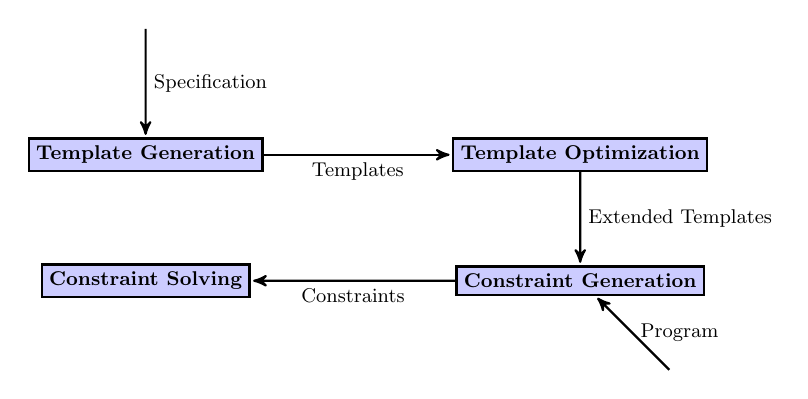
\begin{tikzpicture}[scale=.8,transform shape,->,>=stealth',shorten >=1pt,auto,align=center,node distance=2cm,
  thick,main node/.style={rectangle,fill=blue!20,draw,font=\small\bfseries}]
  \node[main node,fill=\selectTemplateGeneration] (1) {Template Generation};
  \node[main node,fill=\selectTemplateOptimization] (2) [right=3cm of 1] {Template Optimization};
  \node[main node,fill=\selectConstraintGeneration] (3) [below of=2] {Constraint Generation};
  \node[main node,fill=\selectConstraintSolving] (4) [below of=1] {Constraint Solving};
  \coordinate [below right of=3] (5);
  \coordinate [above of=1] (6);

  \path[every node/.style={font=\small}]
    (1) edge node [right, below] {Templates} (2)
    (2) edge node [right] {Extended Templates} (3)
    (5) edge node [right] {Program} (3)
    (3) edge node [right, below] {Constraints} (4)
    (6) edge node [right] {Specification} (1);
\end{tikzpicture}
\caption{Phases of the type checker generator}
\label{fig:phases}
\end{figure}
\end{frame}

\renewcommand*\selectTemplateGeneration{orange}
\againframe{overview}
\renewcommand*\selectTemplateGeneration{}

\defverbatim[colored]\lstApp{%
\begin{lstlisting}
~U = [ %x -> ~S ] ~T
$C1 | $C2 |- ~e : all %x . ~T
============================== T-Tapp
$C1 | $C2 |- ~e [ ~S ] : ~U
\end{lstlisting}
}

\defverbatim[colored]\lstAppRewritten{%
\begin{lstlisting}
$C1 | $C2 |- ~e : all %x . ~T
~U = [ %x -> ~S ] ~T
============================== T-Tapp
$C1 | $C2 |- ~e [ ~S ] : ~U
\end{lstlisting}
}

\defverbatim[colored]\lstSubst{%
\begin{lstlisting}
===================== Subst-Eq
~S = [ %x -> ~S ] %x
\end{lstlisting}
}

\defverbatim[colored]\lstSubstRewritten{%
\begin{lstlisting}
%y = %z
===================== SubstEq
~S = [ %y -> ~S ] %z
\end{lstlisting}
}

\begin{frame}[allowframebreaks, fragile]
  \frametitle{Template Generation}
  \begin{itemize}
  \item Templates are an intermediate representation of the rules
    suitable for constraint generation
  \item An excerpt of the syntax definition of a template:
  \end{itemize}

  \begin{grammar}
    <Template> ::= `Template' $\langle$Premisses$\rangle$ $\langle$Conjecture$\rangle$

    <Conjecture> ::= `Conjecture' $\langle$Judg$\rangle$ $\langle$Name$\rangle$ $\langle$Pattern$\rangle$ $\langle$Outputs$\rangle$

    <Premisses> ::= $\epsilon$ | $\langle$Premise$\rangle$ $\langle$Dependencies$\rangle$ $\langle$Premisses$\rangle$

    <Premise> ::= `Lookup' $\langle$Ctx$\rangle$ $\langle$Inputs$\rangle$ $\langle$Outputs$\rangle$ $\langle$Error$\rangle$
    \alt `Judgment' $\langle$Judg$\rangle$ $\langle$Inputs$\rangle$ $\langle$Binding$\rangle$ $\langle$Outputs$\rangle$ $\langle$Error$\rangle$
    \alt `Eq' $\langle$Term$\rangle$ $\langle$Term$\rangle$ $\langle$Error$\rangle$
    \alt `Neq' $\langle$Term$\rangle$ $\langle$Term$\rangle$ $\langle$Error$\rangle$

    <Dependencies> ::= $\epsilon$ | $\langle$Judg$\rangle$ $\langle$Outputs$\rangle$ $\langle$Dependencies$\rangle$
  \end{grammar}
\end{frame}

\begin{frame}[fragile]
  \frametitle{Template Generation II}
\begin{itemize}
\item Resolve Dependencies between premisses
\item Resolve implicit equalities
\end{itemize}

\begin{lstlisting}
judgments
TermBinding{I} "|" TypeBinding{I} "|-" Exp{I} ":" Type{O}.
Type{O} "= [" ID{I} "->" Type{I} "]" Type{I}.
\end{lstlisting}

\only<1>{\lstApp}
\only<2->{\lstAppRewritten}
\only<1,2>{\lstSubst}
\only<3->{\lstSubstRewritten}
\end{frame}

\renewcommand*\selectTemplateOptimization{orange}
\againframe{overview}
\renewcommand*\selectTemplateOptimization{}

\begin{frame}[allowframebreaks, fragile]
  \frametitle{Template Optimization}
  \begin{itemize}
  \item In contrast to the rules templates are normalized
  \item Templates can still contain redundancies and
    non-syntax-directed rules
  \item We use a first-order formula representation of the templates
    to proof properties that allow to remove redundancies and to make
    rule syntax directed
  \item The first-order formula representation of a template looks
    roughly like this
    \begin{align}
      \forall FV(p_1,\dots, p_n, c) .& p_1 \land \dots \land p_n
      \implies c
    \end{align}
    where $p_i$ and $c$ are propositions representing the premisses
    respectively the conclusion.
  \end{itemize}

\framebreak{}

  \begin{itemize}
  \item A template is \textit{when-ambiguous} if there is an other
    template such that there is at least one term that matches the
    conclusion of both templates.
  \item If the set of terms is equal, we call the ambiguity
    \textit{which-ambiguity}.
\begin{figure}
\begin{verbatim}
~T <: ~S
{ $R } <: { $U }
=============================== S-depth
{ %l : ~T $R } <: { %l : ~S $U }

{ $R } <: { $S }
=============================== S-width
{ %l : ~T $R } <: { %l : ~T $S}
\end{verbatim}
\caption{Which-ambiguity between depth and width subtyping rules of records}
\end{figure}
\end{itemize}
\end{frame}


\begin{frame}
  \frametitle{References}
  \bibliographystyle{amsalpha}
  \bibliography{../report/bibliography.bib}
\end{frame}

\end{document}